\section{Smoothing}
\subsection{Task a}

In this part, mainly use the code from HA3 Q3, but use \texttt{nonLinRTSsmoother} function to generate the filtered output and the smoothed output.

And I realized my last HA3 had some bug, after the fix, the tuning value is chosen as :

\begin{equation}
    \begin{aligned}
        sigma_v = 10;\\
sigma_w = pi/180*6;\nonumber
    \end{aligned}
\end{equation}

The result shown in figure \ref{taska}, legends are detailed. To be more readable and to concentrate on the differences, the picture is zoomed in:

\begin{figure}[H]
 \centering
 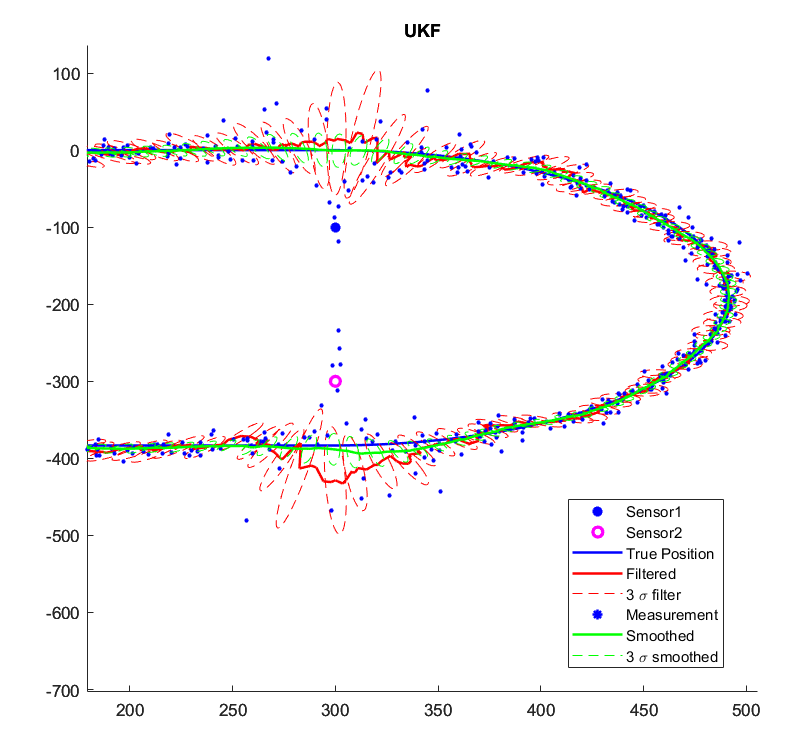
\includegraphics[width=0.7\textwidth]{images/taska.png}
 \caption{Task a: Comparison}
 \label{taska}
\end{figure}

\subsubsection{Conclusion}

From figure \ref{taska}, the green curve, which represents the smoothed output is closer to the true position line compare with the red curve, which represents the filtered output.

And from the $ 5_{th} $ curves, the covariances of the smoothed output are smaller than the filtered one.

\subsection{Task b}

I increased the value at $k=300$  by $ 10\% $ when generating true state $ X $ to see the result:

\begin{lstlisting}
    for i = 2:K+1
    if i ==300
    X(:,i) = 1.1*coordinatedTurnMotion(X(:,i-1),T);
    X(5,i) = 1.1*omega(i);
    else
    X(:,i) = coordinatedTurnMotion(X(:,i-1),T);
    X(5,i) = omega(i);
    end
end
\end{lstlisting}

\begin{figure}[H]
 \centering
 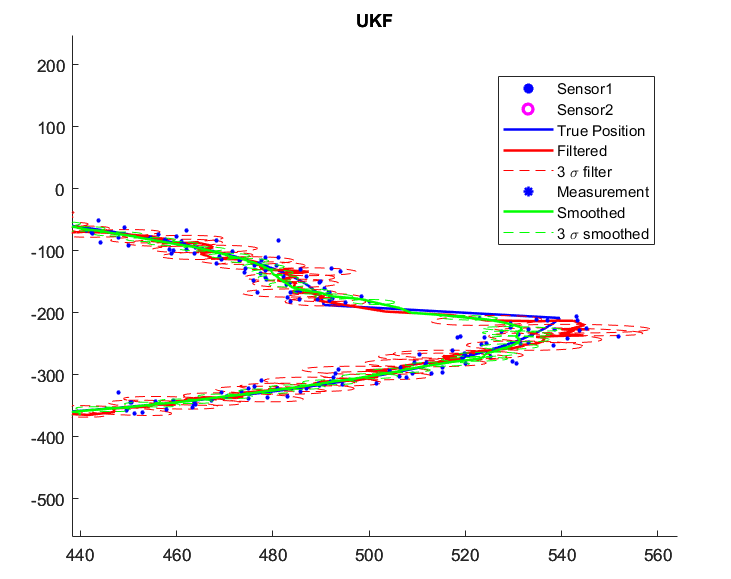
\includegraphics[width=0.7\textwidth]{images/taskb.png}
 \caption{Task b: Manually outlier}
 \label{Taskb}
\end{figure}

From figure \ref{Taskb}, the filtered output of the red curve follows the change of my manual outlier value, and has a big covariance at that point, while the smoothed output of the green curve goes less to the wrong value and has a smaller covariance compare to the filtered curve.

In summary, the filter is trying to incorporate the most recent measurement, including the outlier, into its estimate, while the smoother takes into account both past and future measurements when updating its estimate. As a result, the smoother can mitigate the effect of the outlier by considering the overall trajectory of the object and recognizing that the outlier is inconsistent with the other measurements.